\documentclass[11pt,article]{article}
\usepackage[utf8]{inputenc}
\usepackage[T1]{fontenc} % caractères accentués en entrée, dans emacs
\usepackage[french]{babel}
\FrenchFootnotes
\selectlanguage{french}
\usepackage{a4wide} % possibilité d'utiliser toute la page a4
% selon GUT#33, avril 2007, page 13, empagement
% largeur des textes (ou justification) = 15cm
% hauteur du rectangle d'empagement = 23cm
% blanc de couture = 2/5 (21-15) = 2.4 = inner = right
% blanc de grand fond = 3/5 (21-15) = outer = left
% blanc de tête = 2/5 (29,7-23) = top
% blanc de pied = 3/5 (29,7-23) = bottom
%\usepackage[a4paper,twoside=true,right=2.4cm,left=3.6cm,top=2.68cm,bottom=4.02cm]{geometry}
% selon CFSE 2006
% - largeur des textes (ou justification) : 16cm (2cm de marge, et 1cm
%   de reliure) ;
% - hauteur des textes, y compris les notes : 23cm (2,5cm de marge
%   haute et 2cm de marge basse) ; 1ère page de : 36pts
%   d'espacement avant le titre ;
\oddsidemargin   -4mm           % 3cm a gauche des impaires
\evensidemargin   4mm           % 2cm a gauche des paires
\topmargin       -18mm          % 2.5cm en haut
\headheight       13mm          % taille de l'entete (lignes)
\headsep          24pt          % espace entre entete et texte
\footskip         30pt          % espace entre pied de page et texte
\textheight      230mm          % longeur du texte
\textwidth       160mm          % largeur du texte
\parskip 1pt                    % pas de sauts entre paragraphes
%\parindent 0pt                  % largeur de l'indentation
\usepackage{graphicx} % figure postcript avec latex,
		      % figure png avec pdflatex, au lieu d'utiliser epsfig
\usepackage[usenames,dvipsnames,table]{xcolor}
\usepackage{paralist}
\usepackage{ifthen}
\usepackage{amssymb}
\usepackage{amsfonts}
\usepackage{amsmath}
\usepackage{eurosym}
\usepackage{textcomp}
\usepackage{listings}
\lstset{language=Java,numbers=left,numberstyle=\tiny,stepnumber=4,numbersep=5pt,xleftmargin=5pt}

\usepackage{alltt}
\usepackage{longtable}

% adjust word spacing less strictly
% as result, some spaces between words may be a bit too large,
% but long words will be placed properly.
\sloppy

\newcommand{\cmt}[1]{\texttt{<}\textbf{--~#1~--}\texttt{>}}

\usepackage{lineno}
\usepackage{xspace}

\setlength{\marginparwidth}{1cm}
\setlength{\marginparsep}{10pt}
\reversemarginpar
\newcounter{usecasehaute}
\newcommand{\haute}{Haute}
\newcommand{\moyenne}{Moyenne}
\newcommand{\basse}{basse}
\newcommand{\usecase}[4]{\item \marginpar{\vspace{5pt}\ifthenelse{\equal{#1}{Haute}}{\centering\textsc{#1}\stepcounter{usecasehaute}\newline n$^{\circ}$ \theusecasehaute}{\ifthenelse{\equal{#1}{Moyenne}}{#1}{\small #1}}} #2 \begin{itemize}\item précondition~: #3 \item postcondition~: #4\end{itemize}}
\newcommand{\priorityusecase}[2]{\item \marginpar{\vspace{5pt}\ifthenelse{\equal{#1}{Haute}}{\centering\textsc{#1}\stepcounter{usecasehaute}\newline n$^{\circ}$ \theusecasehaute}{\ifthenelse{\equal{#1}{Moyenne}}{#1}{\small #1}}} #2}
\newcommand{\casusecase}[4]{\usecase{#1}{#2}{#3}{#4}}

\newcommand{\nullvalue}{\textsf{null}\xspace}
\newcommand{\emptyvalue}{\ensuremath\mathrm{vide}}
\newcommand{\invariant}{\ensuremath\mathrm{invariant}}

\begin{document}
\title{Projet CSC4102: Gestion des clefs dans un hôtel}
\author{DUBOC Aurélien et ZHEN Alice}
\date{Année 2019--2020~---~\today}
\maketitle

\newpage

\tableofcontents

\newpage

\section{Spécification}

\subsection{Diagrammes de cas d'utilisation}

\begin{figure}[h!]
\begin{center}
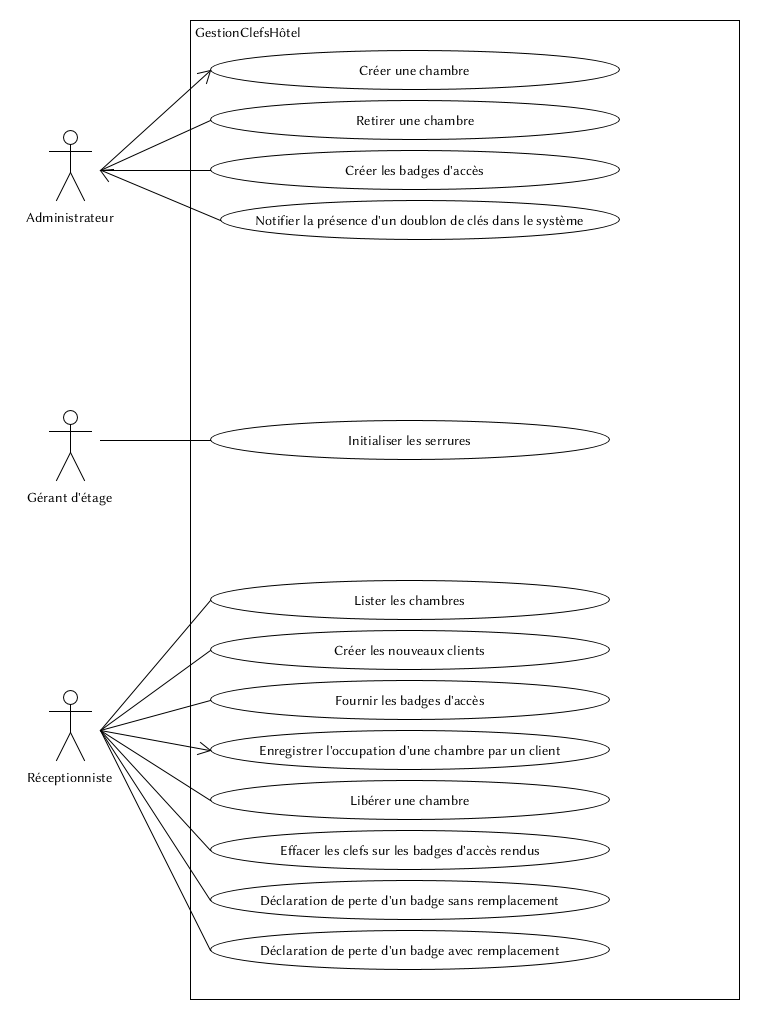
\includegraphics[scale=0.5]{DiagrammesDeCasDUtilisation/gestionclefshotel_uml_diag_cas_utilisation}
\caption{Diagramme de cas d'utilisation}
\end{center}
\label{umlet_diag_cas_utilisation}
\end{figure}

\newpage

\subsection{Priorités, préconditions et postconditions des cas d'utilisation}

Dans la suite, nous donnons les préconditions et postconditions pour
les cas d'utilisation de priorité <<~\haute~>>. Pour les autres, nous
indiquons uniquement leur niveau de priorité.

\bigskip

\begin{compactitem}
\usecase{\haute}{Créer une chambre}
        %% précondition
        {identifiant de la chambre non nul $\land$ chambre avec cet identifiant inexistante $\land$
          graine pour la génération des clefs bien formée (non
          \nullvalue et non vide)}
        %% postcondition
        {chambre avec cet identifiant existante}

\smallskip

\usecase{\haute}{Créer un nouveau client}
        %% précondition
        {client n'existe pas dans le système $\land$ informations personnelles bien formées (non \nullvalue et non vide)}
        %% postcondition
        {client existant dans le système}

\smallskip

\usecase{\haute}{Créer les badges d'accès}
        %% précondition
        {identifiant du badge non nul}
        %% postcondition
        {badge d'accès créé}

\smallskip

\usecase{\haute}{Enregistrer l'occupation d'une chambre par un client}
        %% précondition
        {client existant dans le système $\land$ chambre existante avec ce code $\land$ chambre avec ce code inoccupée}
        %% postcondition
	{client enregistré dans la chambre $\land$ écriture de la nouvelle paire de clés dans le badge d'accès}

\smallskip

\usecase{\haute}{Déclarer la perte d'un badge d'accès sans remplacement}
        %% précondition
        {badge existant dans le système avec cet identifiant}
        %% postcondition
	{clefs du badge en question \nullvalue $\land$ badge marqué comme perdu $\land$ aucune chambre associée à ce badge}

\smallskip

\priorityusecase{\moyenne}{Déclarer la perte d'un badge d'accès avec remplacement}

\smallskip

\priorityusecase{\moyenne}{Fournir les badges d'accès}

\smallskip

\priorityusecase{\moyenne}{Lister les chambres}

\smallskip

\priorityusecase{\basse}{Enregistrer le départ d'un client}

\smallskip

\priorityusecase{\basse}{Retirer une chambre}

\smallskip

\priorityusecase{\basse}{Effacer les clefs sur les badges d'accès rendus}
\end{compactitem}

\newpage

\section{Préparation des tests de validation}

\subsection{Tables de décision des tests de validation}

La fiche programme du module CSC4102 ne permettant pas de développer
des tests de validation couvrant l'ensemble des cas d'utilisation de
l'application, les cas d'utilisation choisis sont de priorité
\textsc{Haute}.

\begin{table}[htbp!]
\begin{tabular}{|p{0.6\linewidth}|c|c|c|c|}
\hline
Numéro de test
&1&2&3&4\\
\hline
\hline
Identifiant de la chambre non nul
&F&T&T&T\\
\hline
Graine pour la génération des clefs bien formée ($\neq$ \nullvalue $\land$ $\neq$ vide)
& &F&T&T\\
\hline
Chambre inexistante avec ce code
& & &F&T\\
\hline
\hline
Création acceptée
&F&F&F&T\\
\hline
\hline
Nombre de jeux de test
&1&2&1&1\\
\hline
\end{tabular}
\caption{Cas d'utilisation <<~créer une chambre~>>}
\end{table}

\begin{table}[htbp!]
\begin{tabular}{|p{0.6\linewidth}|c|c|c|c|c|c|}
\hline
Numéro de test
&1&2&3&4&5&6\\
\hline
\hline
Identifiant du client non nul
&F&T&T&T&T&T\\
\hline
Client existant dans le système
& &F&T&T&T&T\\
\hline
Identifiant de la chambre non nul
& & &F&T&T&T\\
\hline
Chambre existante avec ce code
& & & &F&T&T\\
\hline
Chambre avec ce code inoccupée
& & & & &F&T\\
\hline
\hline
Client enregistré dans la chambre
&F&F&F&F&F&T\\
\hline
\hline
Nombre de jeux de test
&1&1&1&1&1&1\\
\hline
\end{tabular}
\caption{Cas d'utilisation <<~enregistrer l'occupation d'une chambre par un client~>>}
\end{table}

\begin{table}[htbp!]
\begin{tabular}{|p{0.6\linewidth}|c|c|c|c|c|c|}
\hline
Numéro de test
&1&2&3&4\\
\hline
\hline
Identifiant de la chambre non nul
&F&T&T&T\\
\hline
Chambre existante avec cet identifiant
& &F&T&T\\
\hline
Chambre avec cet identifiant bien occupée
& & &F&T\\
\hline
\hline
Chambre libérée
&F&F&F&T\\
\hline
\hline
Nombre de jeux de test
&1&1&1&1\\
\hline
\end{tabular}
\caption{Cas d'utilisation <<~libérer une chambre~>>}
\end{table}
\newpage

\begin{table}[htbp!]
\begin{tabular}{|p{0.6\linewidth}|c|c|c|c|c|c|}
\hline
Numéro de test
&1&2&3\\
\hline
\hline
Identifiant du badge non nul
&F&T&T\\
\hline
Badge existant dans le système avec cet identifiant
& &F&T\\
\hline
\hline
Badge marqué comme perdu
&F&F&T\\
\hline
Clefs du badge valant toutes les deux \nullvalue
&F&F&T\\
\hline
Aucune chambre associée à ce badge
&F&F&T\\
\hline
\hline
Nombre de jeux de test
&1&1&1\\
\hline
\end{tabular}
\caption{Cas d'utilisation <<~Déclarer la perte d'un badge d'accès sans remplacement~>>}
\end{table}
\newpage

\section{Conception}

\subsection{Liste des classes}

À la suite d'un parcours des diagrammes de cas d'utilisation et d'une
relecture de l'étude de cas, voici la liste de classes avec quelques
attributs:
\begin{compactitem}
\item \textsf{GestionClefsHotel} (la façade) instance,
\item \textsf{Util} (classe utilitaire déjà programmée)~---~'attribut
  de classe \textsf{TAILLE\_CLEF}, méthodes de classe
  \textsf{genererUneNouvelleClef} et \textsf{clefToString}),
\item \textsf{Clef} hash
\item \textsf{Badge} identifiant, premiereClef, secondeClef, perdu
\item \textsf{Client} identifiant, nom, prénom
\item \textsf{Chambre} identifiant, premiereClef, secondeClef, graine, sel
\end{compactitem}
\newpage

\subsection{Diagramme de classes}

\begin{figure}[h!]
\begin{center}
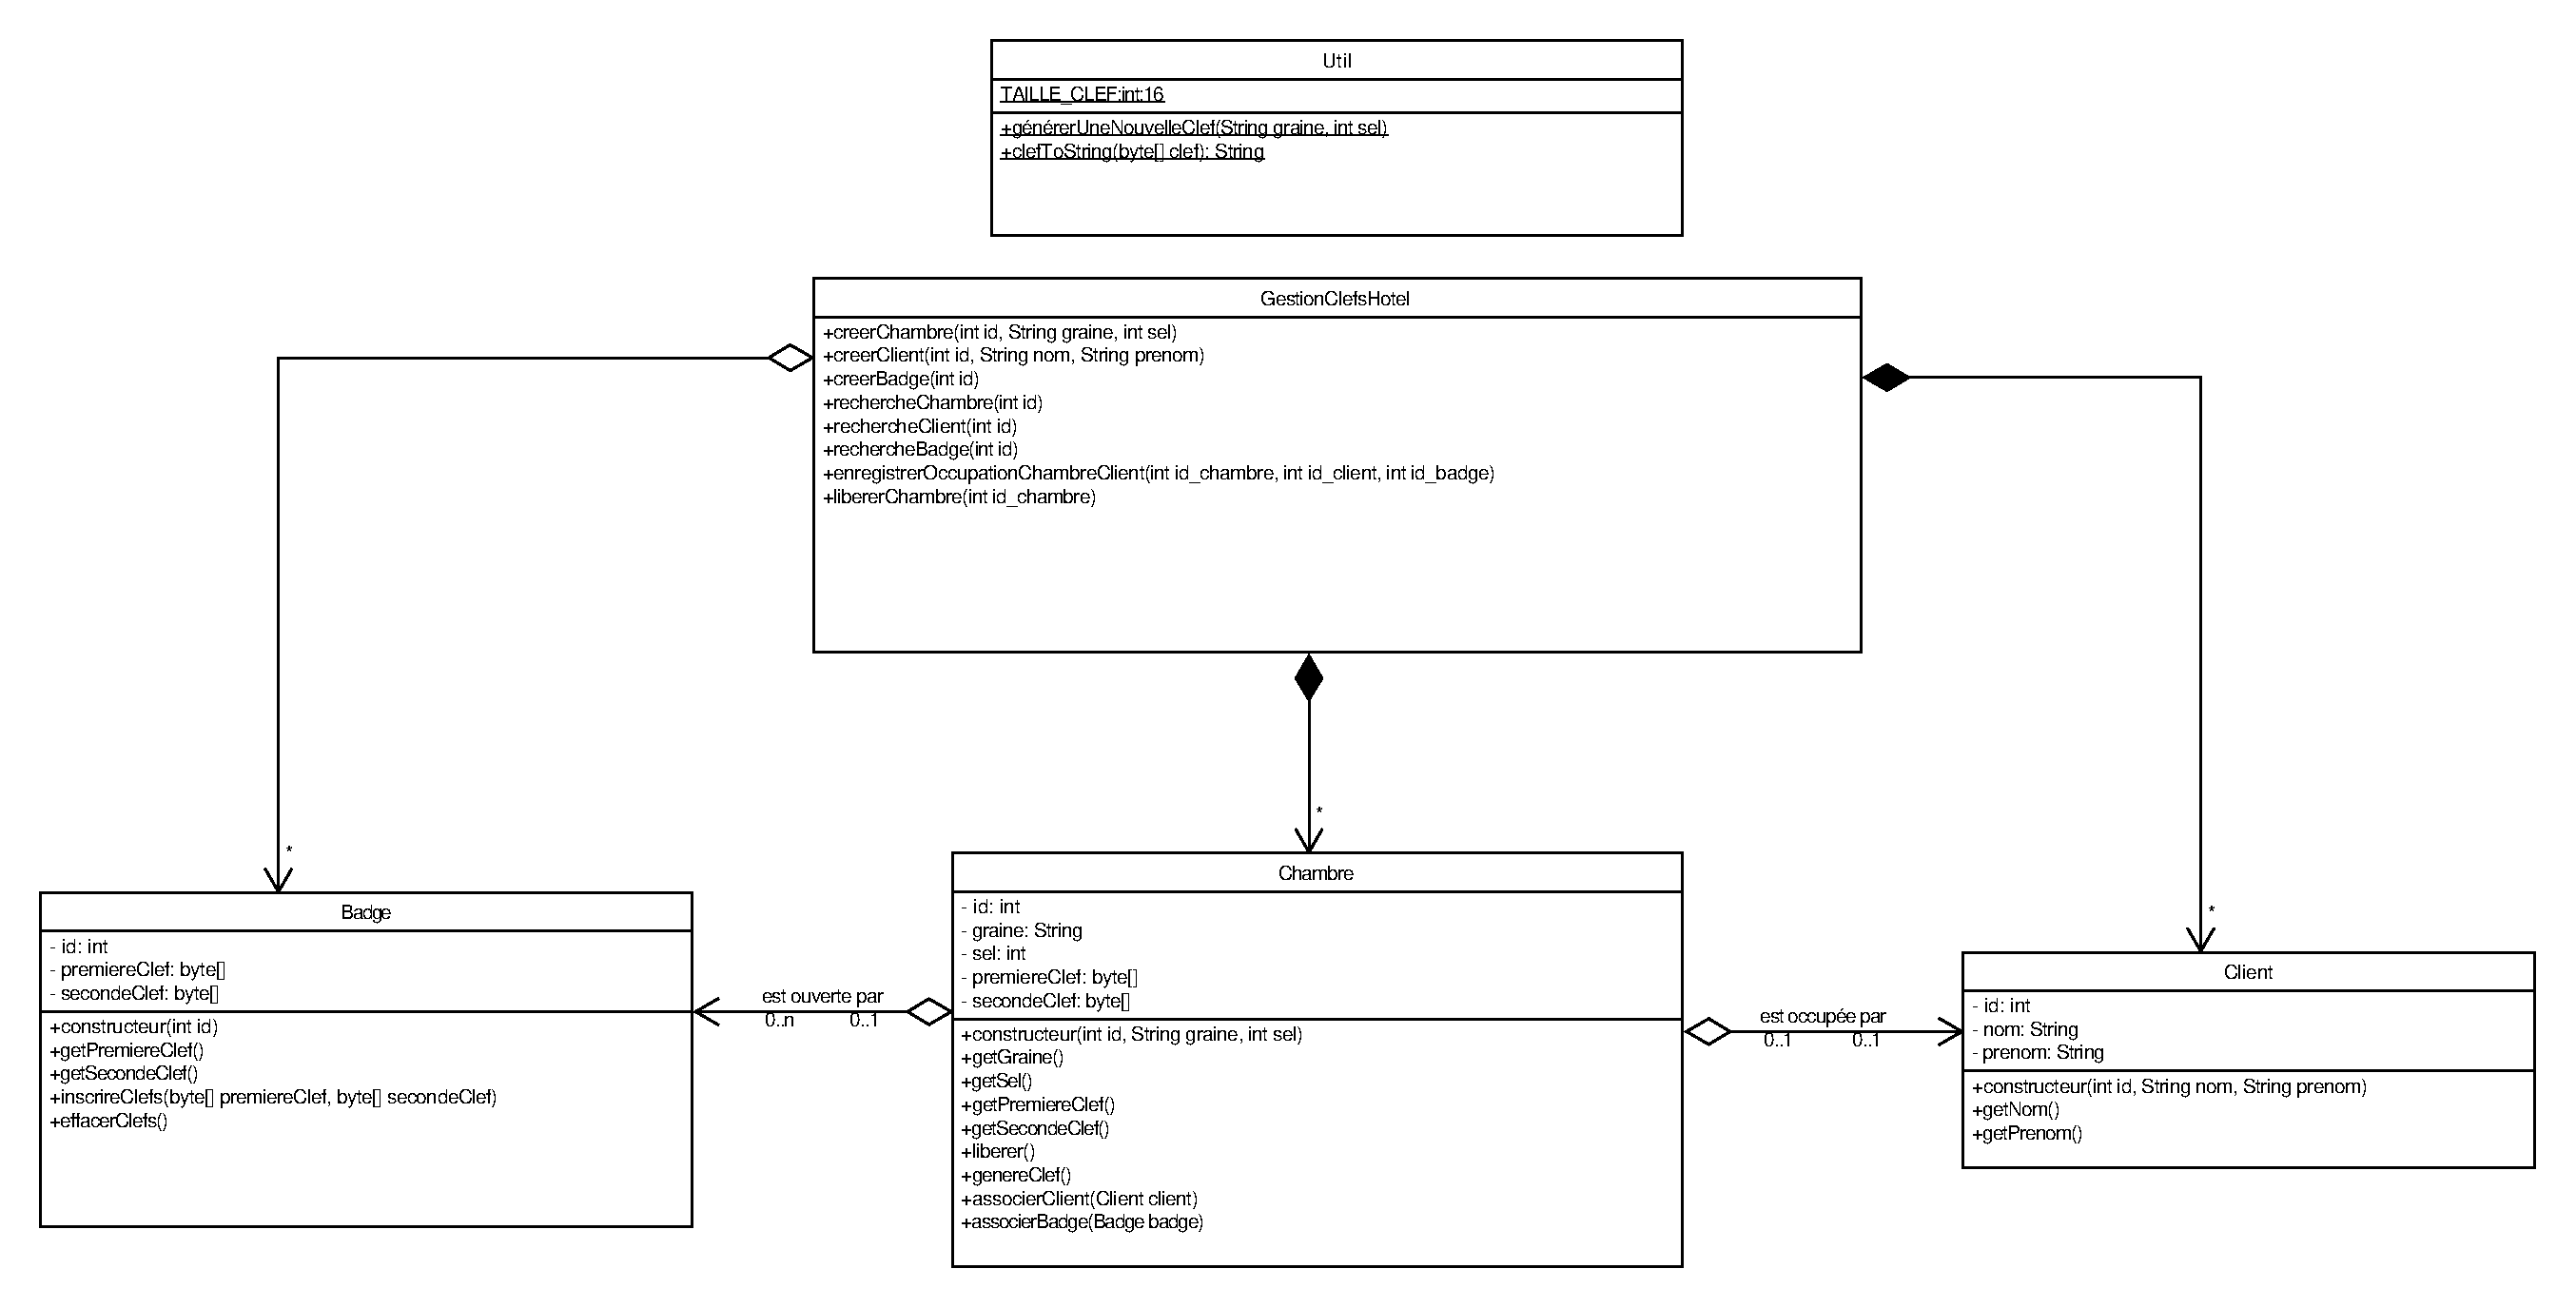
\includegraphics[scale=0.4]{DiagrammesDeClasses/gestionclefshotel_uml_diag_classes}
\caption{Diagramme de classes}
\end{center}
\label{umlet_diag_classes}
\end{figure}

\newpage

\subsection{Diagrammes de séquence}

\begin{figure}[h!]
\begin{center}
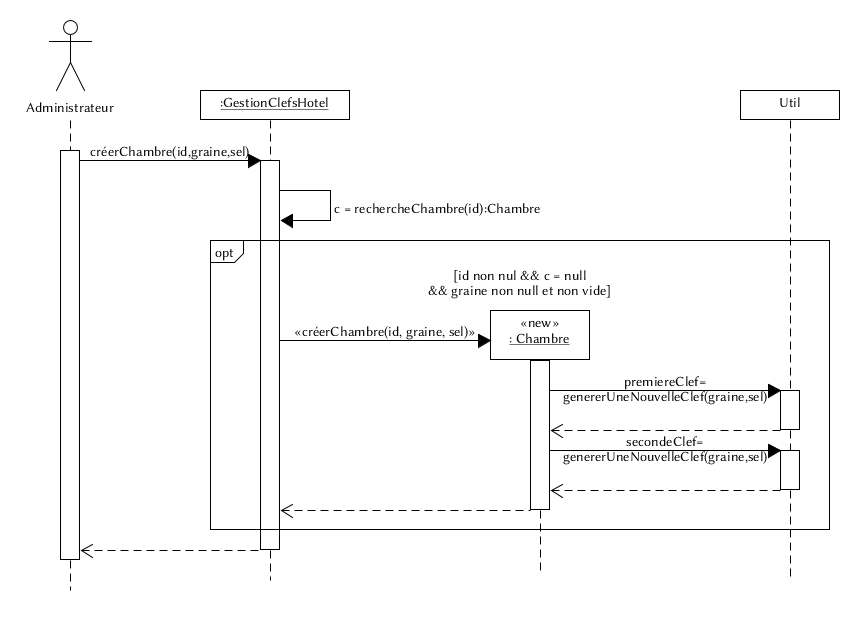
\includegraphics[scale=0.4]{DiagrammesDeSequence/gestionclefshotel_uml_diag_seq_creer_chambre}
\caption{Diagramme de séquence <<~créer une chambre~>>}
\end{center}
\label{umlet_diag_classes}
\end{figure}

\begin{figure}[h!]
\begin{center}
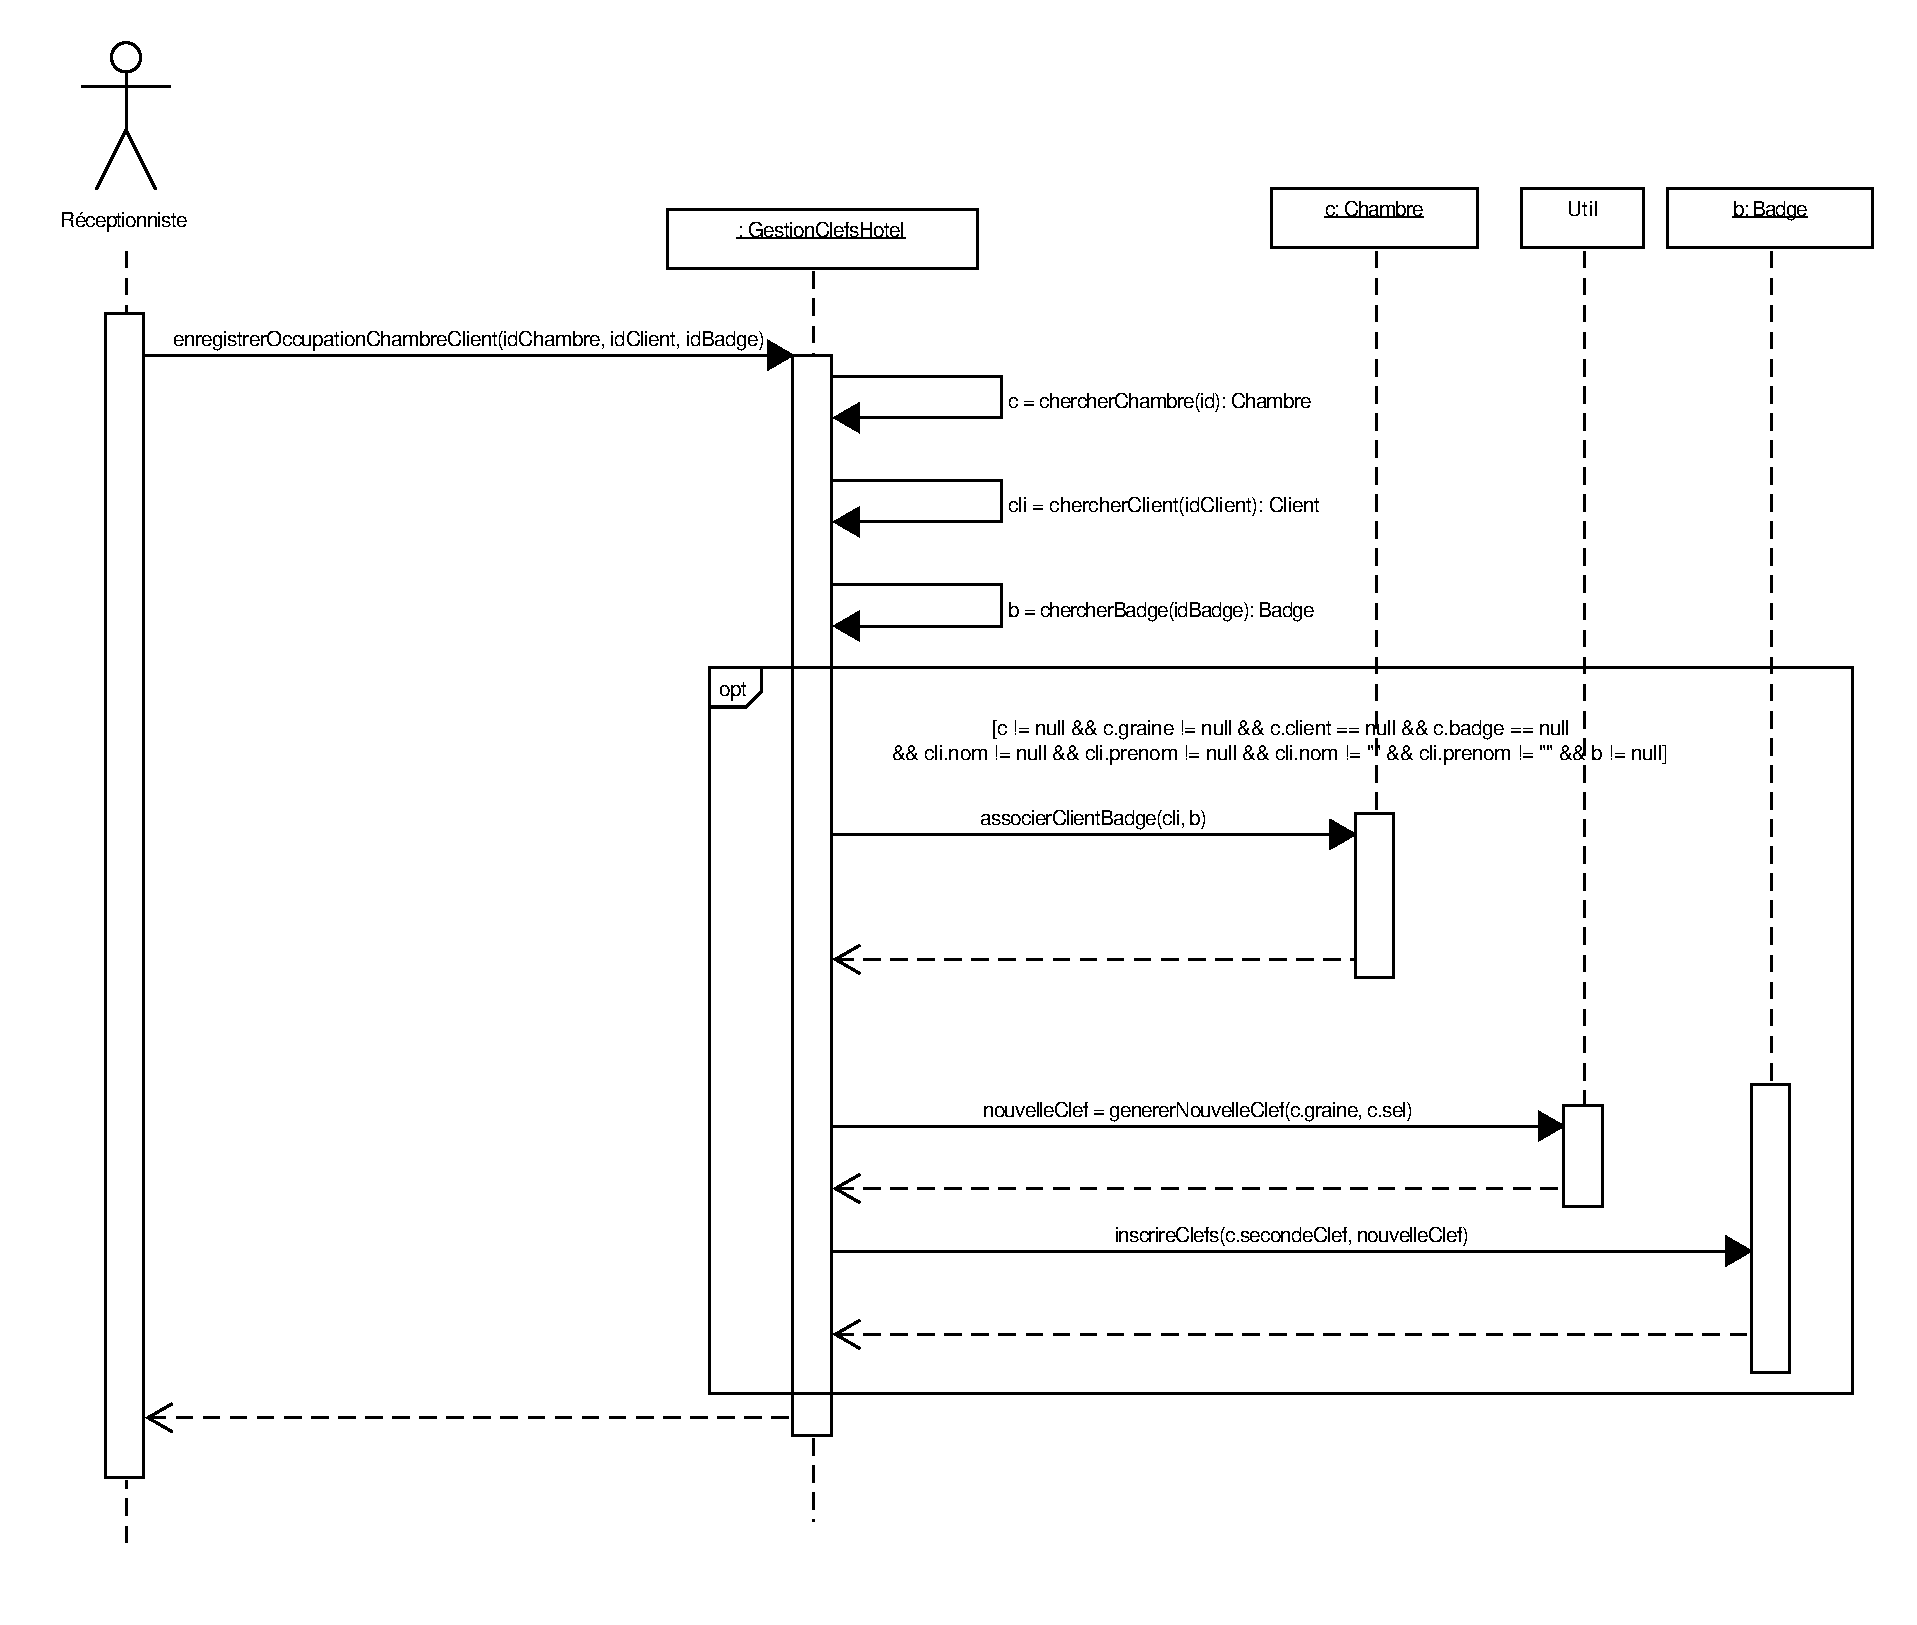
\includegraphics[scale=0.3]{DiagrammesDeSequence/gestionclefshotel_uml_diag_seq_enregistrer_occupation_chambre_client}
\caption{Diagramme de séquence <<~enregistrer l'occupation d'une chambre par un client~>>}
\end{center}
\label{umlet_diag_classes}
\end{figure}

\begin{figure}[h!]
\begin{center}
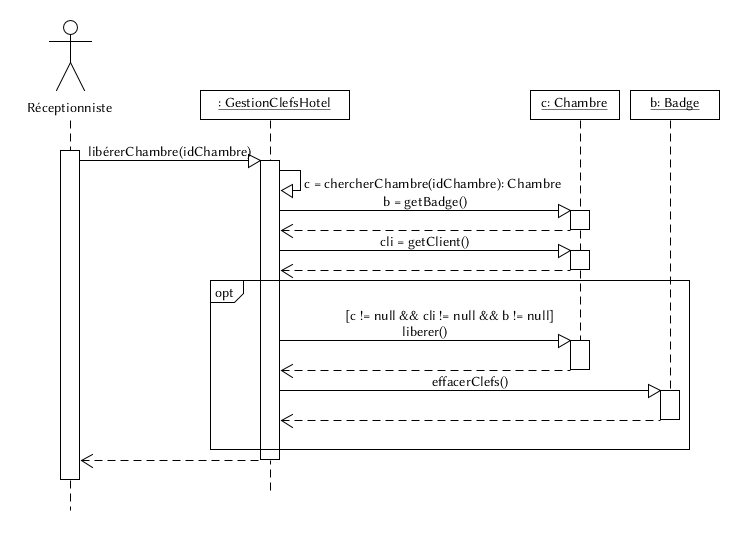
\includegraphics[scale=0.4]{DiagrammesDeSequence/gestionclefshotel_uml_diag_seq_liberer_chambre}
\caption{Diagramme de séquence <<~libérer une chambre~>>}
\end{center}
\label{umlet_diag_classes}
\end{figure}

\begin{figure}[h!]
\begin{center}
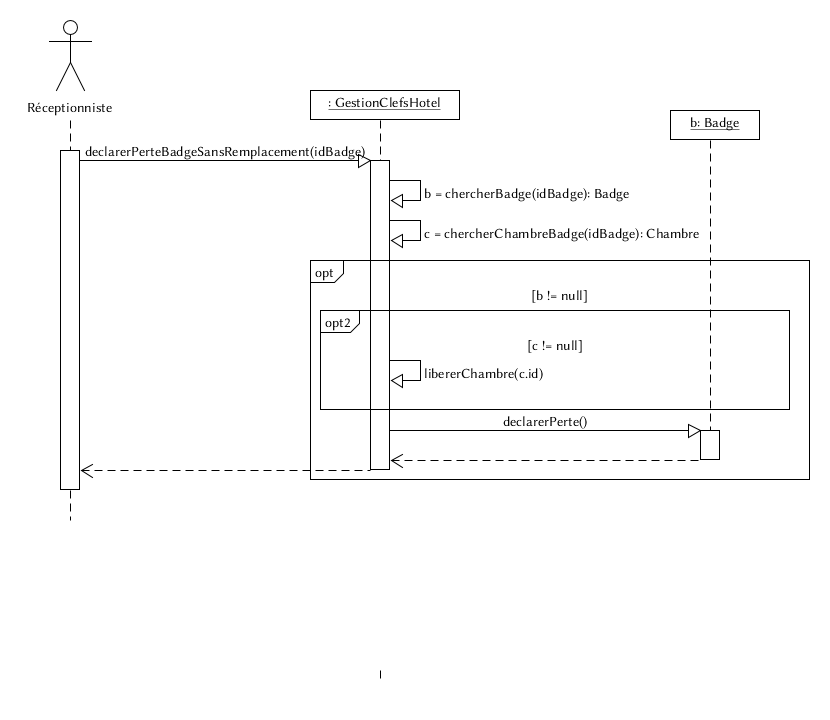
\includegraphics[scale=0.4]{DiagrammesDeSequence/gestionclefshotel_uml_diag_seq_declarer_perte_badge_sans_remplacement}
\caption{Diagramme de séquence <<~déclarer la perte d'un badge sans remplacement~>>}
\end{center}
\label{umlet_diag_classes}
\end{figure}

\clearpage
\newpage

\section{Fiche des classes}

\subsection{Classe \textsf{GestionClefsHotel}}

\begin{center}
\begin{longtable}{|p{15cm}|}
\hline
\multicolumn{1}{|c|}{{\Large \textsf{GestionClefsHotel}}} \\
\hline
%\cmt{attributs}\\
\cmt{attributs <<~association~>>}\\
$-$ chambres : collection de @Chambre \\
$-$ clients : collection de @Client \\
$-$ badges : collection de @Badge \\
$-$ instance : GestionClefsHotel
\hline
\cmt{constructeur} \\
$-$ GestionClefsHotel()\\
$+$ getInstance() : GestionClefsHotel\\
$+$ reset()\\
$+$ invariant() : booléen\\
\cmt{operations <<~cas d'utilisation~>>} \\
$+$ créerChambre(int id, String graine, int sel) \\
$+$ créerClient(int id, String nom, String prenom) \\
$+$ créerBadge(int id) \\
$+$ enregistrerOccupationChambreClient(int id\_chambre, int id\_client, int id\_badge) \\
$+$ libérerChambre(int id\_chambre) \\
$+$ déclarerPerteBadgeSansRemplacement(int id\_badge) \\
$+$ déclarerPerteBadgeAvecRemplacement(int id\_badge) \\
\cmt{opérations de recherche} \\
$+$ chercherChambre(int id) : Chambre \\
$+$ chercherClient(int id) : Client\\
$+$ chercherBadge(int id) : Badge\\
$+$ chercherChambreBadge(int id\_badge) : Chambre \\
\hline
\end{longtable}%)
\end{center}
\clearpage
\newpage

\subsection{Classe \textsf{Badge}}

\begin{center}
\begin{longtable}{|p{15cm}|}
\hline
\multicolumn{1}{|c|}{{\Large \textsf{Badge}}} \\
\hline
\cmt{attributs}\\
$-$ id : int \\
$-$ premiereClef : byte[] \\
$-$ secondeClef : byte[] \\
$-$ perdu : booléen \\
\hline
\cmt{constructeur} \\
$+$ Badge(int id)\\
%$+$ destructeur()\\
$+$ invariant() : booléen\\
\cmt{operations <<~cas d'utilisation~>>} \\
$+$ getId() : int \\
$+$ getPremiereClef() : byte[] \\
$+$ getSecondeClef() : byte[] \\
$+$ estPerdu() : booléen \\
$+$ inscrireClefs(byte[] premiereClef, byte[] secondeClef) \\
$+$ effacerClefs() \\
$+$ déclarerPerte() \\
\hline
\end{longtable}
\end{center}
\clearpage
\newpage

\subsection{Classe \textsf{Chambre}}

\begin{center}
\begin{longtable}{|p{15cm}|}
\hline
\multicolumn{1}{|c|}{{\Large \textsf{Chambre}}} \\
\hline
\cmt{attributs}\\
$-$ id : int \\
$-$ graine : String \\
$-$ sel : int \\
$-$ premiereClef : byte[] \\
$-$ secondeClef : byte[] \\
\cmt{attributs <<~association~>>}\\
$-$ badge : @Badge \\
$-$ client : @Client \\
\hline
\cmt{constructeur} \\
$+$ Chambre(int id, String graine, int sel)\\
%$+$ destructeur()\\
$+$ invariant() : booléen\\
\cmt{operations <<~cas d'utilisation~>>} \\
$+$ getId() : int \\
$+$ getGraine() : String \\
$+$ getSel() : int \\
$+$ getPremiereClef() : byte[] \\
$+$ getSecondeClef() : byte[] \\
$+$ libérer() \\
$+$ genereClef() : byte[] \\
$+$ associerClientBadge(Client client, Badge badge) \\
\hline
\end{longtable}
\end{center}
\newpage

\section{Diagrammes de machine à états et invariants}

\begin{figure}[h!]
\begin{center}
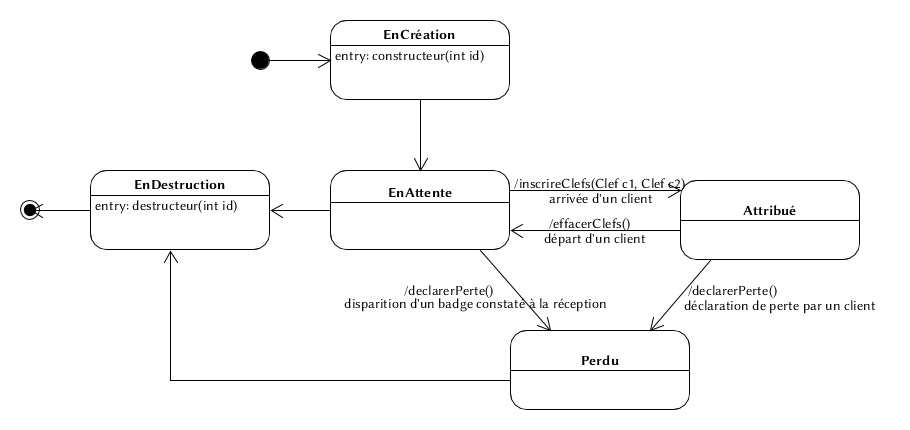
\includegraphics[scale=0.5]{DiagrammesDeMachineAEtats/gestionclefshotel_uml_diag_machine_a_etats_badge}
\caption{Diagramme de machine à états de la classe <<~badge~>>}
\end{center}
\label{umlet_diag_classes}
\end{figure}

\textbf{Invariant de la classe Badge:} (id non nul) \&\& $(/estAttribue \land premiereClef \neq \nullvalue \land secondeClef \neq \nullvalue)$  || $(/nonAttribue \land premiereClef = \nullvalue \land secondeClef = \nullvalue)$

\newpage

\section{Préparation des tests unitaires}

\begin{table}[!ht]
\begin{center}
\begin{tabular}{|p{0.4\linewidth}|c|c|c|}
\hline
Numéro de test
&1&2&3\\
\hline
\hline
Identifiant du badge non nul
&F&T&T\\
\hline
Badge inexistant avec cet identifiant
& &F&T\\
\hline
\hline
$/enAttente = true$
& & &T\\
\hline
$/estAttribue = false$
& & &T\\
\hline
$\invariant$
& & &T\\
\hline
Levée d'une exception&\textsc{oui}&\textsc{oui}&\textsc{non}\\
\hline
\hline
Création du badge acceptée
&F&F&T\\
\hline
\hline
Nombre de jeux de test
&1&1&1\\
\hline
\end{tabular}
\end{center}
\caption{Table de décision des opérations pour Badge <<~constructeur~>>}
\end{table}

\begin{table}[!ht]
\begin{center}
\begin{tabular}{|p{0.4\linewidth}|c|c|}
\hline
Numéro de test
&1&2\\
\hline
\hline
/enAttente
&F&T\\
\hline
\hline
$/enAttente = false$
& &T\\
\hline
$/estAttribue = true$
& &T\\
\hline
$\invariant$
& &T\\
\hline
Levée d'une exception&\textsc{oui}&\textsc{non}\\
\hline
\hline
Attribution du badge confirmée
&F&T\\
\hline
\hline
Nombre de jeux de test
&1&1\\
\hline
\end{tabular}
\end{center}
\caption{Table de décision des opérations pour Badge <<~estAttribué~>>}
\end{table}


\end{document}
